\documentclass{article}
\usepackage{graphicx} % Required for inserting images
\usepackage[top=0.9in, bottom=1in, left=1.5in, right=1.5in]{geometry}
\usepackage[utf8]{inputenc}
\usepackage[icelandic]{babel}
\usepackage[T1]{fontenc}
\usepackage[sc]{mathpazo}
\usepackage[parfill]{parskip}
% Tables and lists
\usepackage{booktabs,tabularx}
\usepackage{multirow}
\usepackage{enumerate}
\usepackage{adjustbox}
\usepackage{multicol}
\usepackage{xcolor}
\usepackage{algpseudocode}
\usepackage{tikz}
\usetikzlibrary{arrows, positioning, calc}

% Math
\usepackage{amsmath, amsfonts, amssymb, amsthm}
% Graphics

\usepackage{graphicx}
\usepackage{tikz}
% Code environment
\usepackage{minted}
%\usepackage{bm}
%\usepackage{siunitx}
%\usepackage{animate}
%\usepackage{hyperref}
%\usepackage{movie15}
%\usepackage{multicol}
%\usepackage{changepage}
\title{Tölvutækni og Forritun Heimadæmi 3}
\author{Ragnar Björn Ingvarsson, rbi3}


\begin{document}
	
	\maketitle
	
	\section{}
	\begin{minipage}{5cm}
		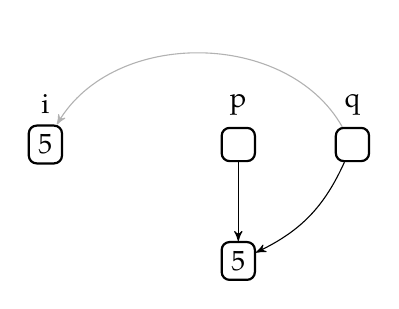
\begin{tikzpicture}[->, >=stealth',
		cube/.style={rectangle,draw=black,
		thick, rounded corners=1mm, minimum size=1.2em}]
		\node[cube] (5) {5};
		\node[cube, above=0.01 of 5, draw=white] (i) {i};
		\node[cube, right=2 of 5] (p*) {};
		\node[cube, above=0.01 of p*, draw=white] (p) {p};
		\node[cube, right=of p*] (q*) {};
		\node[cube, above=0.01 of q*, draw=white] (q) {q};
		\node[cube, below=of p*] (t*) {5};

		\path (p*) edge node {} (t*);
		\path (q*) edge[bend left=20] node {} (t*);
		\path (q*) edge[bend right=60, draw=black!30] node {} (5);

	\end{tikzpicture}
\end{minipage}
\begin{minipage}{9cm}
Svo \texttt{i=5}, \texttt{p} og \texttt{q} benda á ónefnt minnissvæði sem
hefur afritað frá \texttt{i} gildið \texttt{5}.
\end{minipage}

\section{}

\begin{itemize}
	\item[\textbf{a.}]
\begin{verbatim}
#include <stdio.h>
#include <stdlib.h>

int main( int argc, char **argv ) {
	int inntala;

	while (scanf("%d", &inntala) != EOF) {
		printf("%d\n", inntala+1);
	}

	return 0;
}
\end{verbatim}
	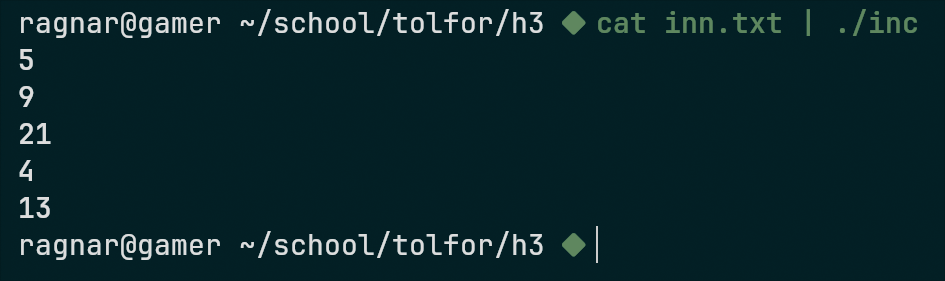
\includegraphics[scale=0.3]{inc.png}
	\newpage
\item[\textbf{b.}]
\begin{verbatim}
#include <stdio.h>
#include <stdlib.h>

int main( int argc, char **argv ) {
	int inntala;

	while (scanf("%d", &inntala) != EOF) {
		printf("%d\n", inntala + atoi(argv[1]));
	}

	return 0;
}
\end{verbatim}
	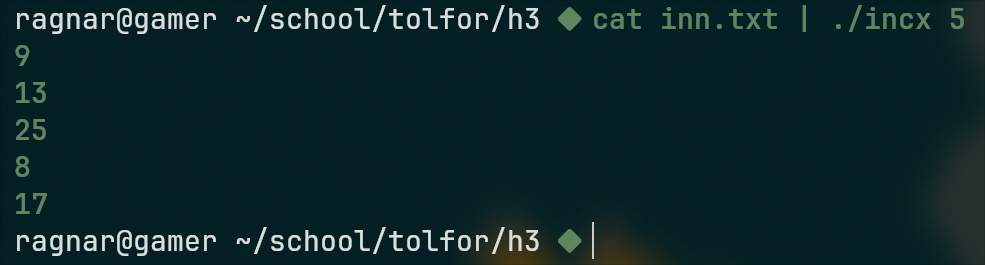
\includegraphics[scale=0.3]{incx.png}
\end{itemize}

\section{}
\begin{verbatim}
int* doubleArr(int* a, int n) {

    /***** Þennan hluta skrifið þið *****/

	int *b = (int *)calloc(n*2, sizeof(int));
	for ( int i = 0; i < n; i++ ) {
		b[i] = a[i];
	}
	free(a);

    /* Skilum hér bendi á upphaflega fylkið til að
       beinagrindin keyri, en gæti þurfa að breyta    */
    return b;
}
\end{verbatim}
\begin{center}
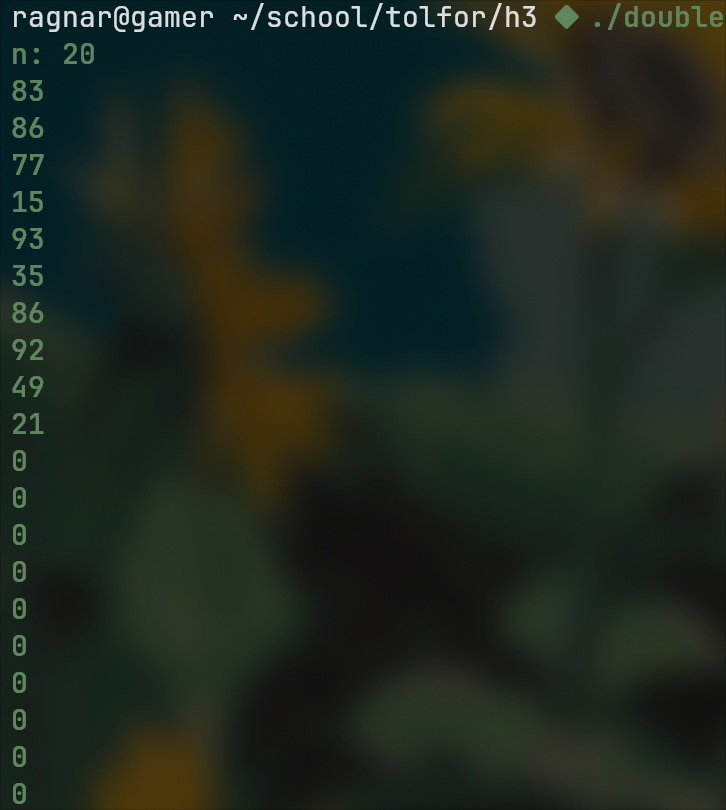
\includegraphics[scale=0.25]{double.png}
\end{center}

\section{}

\begin{verbatim}
#include <stdio.h>
#include <stdlib.h>
#include <string.h>

int main( int argc, char **argv ) {
	int count = 0;
	for ( int i = 1; i < argc; i++ ) {
		count += strlen(argv[i]); 
	}

	char *cat = (char *)calloc(count, sizeof(char));

	for ( int i = 1; i < argc; i++ ) {
		strcat(cat, argv[i]);
	}

	printf("Length is: %i\n", count);
	printf("Concatenation: %s\n", cat);
	return 0;
}
\end{verbatim}

\begin{center}
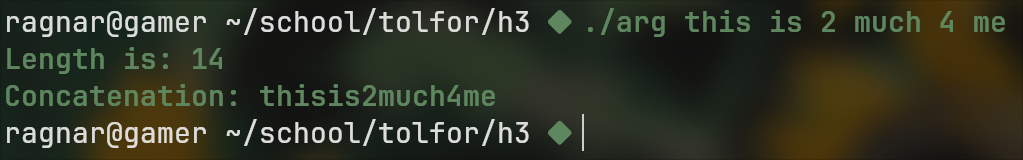
\includegraphics[scale=0.3]{arg.png}
\end{center}

\section{}

\begin{itemize}
	\item[a.]
		\begin{verbatim}
void printRevList() {

    /***** Þið skrifið þennan hluta *****/
	struct dNode *p = tail;

	printf("RevListi: ");
	while (p != NULL) {
		printf("%d ", p->data);
		p = p->prev;
	}
	printf("\n");
}
		\end{verbatim}
	\item[b.]
		\begin{verbatim}
void insAs(int k, int v) {
    struct dNode *p, *q;
    int i;

    /* Búa til hnútinn og setja gildið inn í hann */
    p = (struct dNode *)malloc(sizeof(struct dNode));
    p->data = v;
    
    if (head == NULL) {
        /* Tómur listi */

        /***** Skrifið kóða hér *****/
		head = p;

    } else if (k == 0) {
        /* innsetning fremst í listann */

        /***** Skrifið kóða hér *****/
		p->next = head;
		head->prev = p;
		head = p;

    } else {
        /* annars rekja okkur eftir listanum */


        /***** Skrifið kóða hér *****/
        /* Athugið að hér gæti þurft að uppfæra tail-bendinn */

		int end = 0;
		q = head;
		for ( int i = 0; i < k; i++ ) {
			p->prev = q;
			if ( q->next == NULL ) {
				tail = p;
				end = 1;
				break;
			} else {
				q = q->next;
			}
		}
		(p->prev)->next = p;
		if ( !end ) {
			p->next = q;
			q->prev = p;
		}
   }
}
		\end{verbatim}

\begin{center}
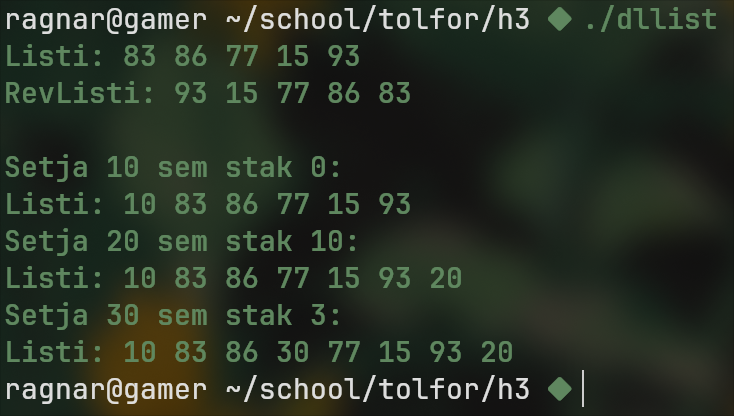
\includegraphics[scale=0.3]{dllist.png}
\end{center}
\end{itemize}

\end{document}
